%\documentclass[times, 10pt, twocolumn]{article} 
%\documentclass[conference,final]{IEEEtran}
     
\documentclass{rspublic}   

%------------------------------------------------------------------------- 
% take the % away on next line to produce the final camera-ready version 
%\pagestyle{empty}

\usepackage[utf8]{inputenc}
\usepackage{graphicx}
\usepackage{url}
\usepackage{float}
\usepackage{times}    
\usepackage{multirow}    
\usepackage{listings}   
\usepackage{times}     
\usepackage{paralist}    
\usepackage{wrapfig}    
\usepackage[small,it]{caption}
\usepackage{multirow}
\usepackage{ifpdf}    
\usepackage{subfig} 
\usepackage{pdfsync}                    
%\usepackage{subfigure}

%Bibliography                     
\usepackage{natbib}   

\usepackage{listings}
\usepackage{keyval}  
\usepackage{color}
\definecolor{listinggray}{gray}{0.95}
\definecolor{darkgray}{gray}{0.7}
\definecolor{commentgreen}{rgb}{0, 0.4, 0}
\definecolor{darkblue}{rgb}{0, 0, 0.4}
\definecolor{middleblue}{rgb}{0, 0, 0.7}
\definecolor{darkred}{rgb}{0.4, 0, 0}
\definecolor{brown}{rgb}{0.5, 0.5, 0}

\lstdefinestyle{myListing}{
  frame=single,   
  backgroundcolor=\color{listinggray},  
  %float=t,
  language=C,       
  basicstyle=\ttfamily \footnotesize,
  breakautoindent=true,
  breaklines=true
  tabsize=2,
  captionpos=b,  
  aboveskip=0em,
  %numbers=left, 
  %numberstyle=\tiny
}      

\lstdefinestyle{myPythonListing}{
  frame=single,   
  backgroundcolor=\color{listinggray},  
  %float=t,
  language=Python,       
  basicstyle=\ttfamily \footnotesize,
  breakautoindent=true,
  breaklines=true
  tabsize=2,
  captionpos=b,  
  %numbers=left, 
  %numberstyle=\tiny
}


\title[Adaptive Distributed Replica-Exchange Simulations]{Adaptive Distributed
  Replica-Exchange Simulations}

\author[Luckow, Jha, Kim, Merzky, Schnor]{
  Andr\'e Luckow$^{1}$, Shantenu Jha$^{2,3,4}$, Joohyun Kim$^{2}$, Andre Merzky$^{2}$ and Bettina Schnor$^{1}$\\
  \small{\emph{$^{1}$Institute of Computer Science, Potsdam University, Germany}}\\
  \small{\emph{$^{2}$Center for Computation \& Technology, Louisiana State University, USA}}\\
  \small{\emph{$^{3}$Department of Computer Science, Louisiana State
      University, USA}}\\
  \small{\emph{$^{4}$e-Science Institute, Edinburgh, UK}}\\
}

%\date{}

\def\acknowledgementname{Acknowledgements}
\newenvironment{acknowledgement}%
{\section*{\acknowledgementname}%
\parindent=0pt%
}

\newif\ifdraft
%\drafttrue
\ifdraft
\newcommand{\kimnote}[1]{ {\textcolor{green} { ***JK: #1 }}}
\newcommand{\alnote}[1]{ {\textcolor{blue} { ***AL: #1 }}}
\newcommand{\amnote}[1]{ {\textcolor{magenta} { ***AM: #1 }}}
\newcommand{\jhanote}[1]{ {\textcolor{red} { ***SJ: #1 }}}
\else
\newcommand{\kimnote}[1]{}
\newcommand{\alnote}[1]{}
\newcommand{\amnote}[1]{}
\newcommand{\jhanote}[1]{}
\fi

\newcommand{\I}[1]{\textit{#1}}
\newcommand{\B}[1]{\textbf{#1}}
\newcommand{\T}[1]{\texttt{#1}}

\newcommand{\glidein}[1]{Glide-In }  
\newcommand{\replicaagent}[1]{Replica-Agent }         
\newcommand{\remanager}[1]{RE-Manager }

\begin{document} 


\maketitle    

% \begin{abstract}{Replica-Exchange, SAGA, Migol, Fault Tolerance}  
%   The ability to effectively utilise multiple distributed resources to
%   reduce the time-to-com\-ple\-tion remains a challenge at many levels.
%   We discuss the Replica-Exchange class of applications, which, 
%   due to the loose-coupling of the sub-tasks (replicas),
%   can benefit greatly from utilising as many resources as available.
%   An implementation of a {\it pleasingly-distributed} algorithm such
%   as Replica-Exchange, that is independent of infrastructural details,
%   however, does not exist.  This paper proposes an extensible and
%   scalable framework based on SAGA and Migol that provides a
%   general-purpose, opportunistic mechanism to effectively utilise
%   multiple resources in an infrastructure independent way. By
%   analysing the requirements of the Replica-Exchange algorithm and the
%   challenges of implementing it on real production systems, we propose
%   a new abstraction (BigJob), which forms the basis of the adaptive
%   redistribution and effective scheduling
%   of replicas.
% %  and the effective scheduling of the  multiple sub-tasks.
% \end{abstract}

\begin{abstract}{Replica-Exchange, SAGA, Migol, Fault Tolerance}  
  Due to the loose-coupling of the replicas, Replica-Exchange class of
  algorithms should be able to benefit greatly from utilising as many
  resources as available, but the ability to effectively utilise
  multiple distributed resources to reduce the time-to-com\-ple\-tion
  remains a challenge at many levels.  Additionally, an implementation
  of a {\it pleasingly-distributed} algorithm such as
  Replica-Exchange, which is independent of infrastructural details,
  however, does not exist.  This paper proposes an extensible and
  scalable framework based on SAGA that provides a general-purpose,
  opportunistic mechanism to effectively utilise multiple resources in
  an infrastructure independent way. By analysing the requirements of
  the Replica-Exchange algorithm and the challenges of implementing it
  on real production systems, we propose a new abstraction (BigJob),
  which forms the basis of the adaptive redistribution and effective
  scheduling of replicas.
\end{abstract}
\section{Introduction}

Several classes of applications are well suited for distributed
environments. Probably the best known and most powerful examples are
those that involve an ensemble of decoupled tasks, such as simple
parameter sweep applications~\citep{1239909}.  A slightly more
complicated and challenging class of distributed applications are
those that have a degree of coupling between individual sub-tasks.  An
interesting example of such applications are those based upon the
\emph{Replica-Exchange (RE)}~\citep{hansmann,Sugita:1999rm} algorithm.
RE simulations are used to understand physical phenomena -- ranging
from protein folding dynamics to binding affinity calculations.

%%%%% RE nature of the problem
RE simulations involve the concurrent execution of multiple similar
simulations -- the \emph{replicas}. The coupling between replicas
occurs via periodic exchange attempts between paired replicas. The
exchange is typically infrequent compared to the run-time of each
replica, and is small in terms of communication bandwidth
requirements. Thus RE is {\it prima facie} a perfect algorithm to
exploit distributed resources. We label such a class of algorithms as
{\it pleasingly-distributed}.

%%%%% related work
Most RE implementations are either infrastructure
specific~\citep{Woods:2005nx}, or if using multiple distributed
resources, require prior co-scheduling~\citep{repex_mpig}.
Ref.~\citep{repex_mpig} is an important example of first-generation
Grid applications, wherein the effectiveness of coupling multiple
distributed resources for scientific problems has been demonstrated.
The real power of distributed systems however, arises from adaptive
algorithms and implementations that provide applications with an agile
execution model, and thus the ability to utilise resources
dynamically, as opposed to a static execution model inherited from
parallel and cluster computing.  Unfortunately, the barrier to the
development of such adaptive applications is high and the
infrastructure support is poor.
%for applications with dynamic resource utilisation requirements 
% Therefore, it is not surprisingly that not many adaptive
% applications exist.
Specifically, there is no implementation of an
adaptive RE algorithm, which is both able to effectively and reliably
utilise multiple distributed resources without prior scheduling as
well as being independent of any specific %computational platform or
infrastructure.
                      
%%%%% reference to contribution of escience paper
% To address heterogeneity and failures, which are both inherent
% characteristics of distributed environments, we demonstrated the use
% of the \textit{Simple API for Grid Applications
%   (SAGA)}~\citep{saga_url}, in particular its Checkpoint Recovery
% (CPR) package, and of the Migol middleware~\citep{schnorLuckow08} to
% build a reliable RE application (see~\citet{Luckow:2008la}).  In
% general, SAGA and Migol provide the tools for developing a broad range
% of applications, of which RE is a specific example.  Implementing such
% a framework was an important first-step on the critical-path towards
% developing a framework that can support adaptive RE simulations on
% production-level infrastructure.

%%%%% contributions of this paper  
% In
% general, SAGA and Migol provide the tools for developing a broad range
% of applications, of which RE is a specific example.  Implementing such
% a framework was an important first-step on the critical-path towards
% developing a framework that can support adaptive RE simulations on
% production-level infrastructure.

% To address heterogeneity and failures, which are both inherent
% characteristics of distributed environments, we demonstrated the use
% of the \textit{Simple API for Grid Applications
%   (SAGA)}~\citep{saga_url}, in particular its Checkpoint Recovery
% (CPR) package, and of the Migol middleware~\citep{schnorLuckow08} to
% build a reliable RE application (see~\citet{Luckow:2008la}).  

% Production distributed environments in their current
% incarnation are manifest as an aggregation of multiple
% single-resources, and although there are some initial attempts at
% supporting co-scheduled resources for tightly-coupled simulations
% there are insufficient attempts at supporting a broader range of
% distributed and collective modes of operations, such as required for
% loosely-coupled applications.  For example, 

% Current production infrastructure does not provide efficient {\it
%   ap\-pli\-cation-level} mechanisms for co-ordinated resource
% sharing. 

In this paper we address some of the challenges and performance
bottlenecks encountered when performing RE simulations over multiple
distributed resources, such as the overall slowdown due to
synchronisation arising from the light-coupling and the lack of
co-scheduled resources.  This work builds upon work on the creation of
fault-tolerant framework~\citet{Luckow:2008la}. The unique
contribution of this paper is the implementation of a RE framework
that overcomes the described limitations, by being able to adapt at
runtime to a change in resource availabilities and application
resource requirements.  We present data that validates the claim that
as more resources become available our framework can opportunistically
employ these resources to lead to a reduction in the
time-to-completion of the scientific problem.  The remainder of the
paper is structured as follows: In the next section we provide the
basic ideas behind RE and specifically RE using Molecular Dynamics
(REMD) simulations.  In section~\ref{sec:remd_impl}, we describe the
details of a REMD application implemented using the SAGA/Mi\-gol
framework. Section~\ref{sec:glidein} discusses the new BigJob
abstraction and the SAGA Glide-In framework.  We highlight different
adaptivity strategies for supporting dynamic applications in
section~\ref{sec:adaptivitiy}.  In the subsequent section we discuss
the deployment and results of experiments using the SAGA based RE
framework on the TeraGrid.  We conclude by discussing related work --
which will highlight the unique features of our implementation, and
provide a glimpse of future work in this direction.

% One approach to rectify these deficits
% are system-level abstractions that allow applications to effectively
% utilise distributed resources concurrently.

% The framework utilises the
% \emph{BigJob} abstraction,
% which % in combination with the Glide-In mechanism,
% allows the efficient dispatching of jobs by grouping smaller sub-jobs
% into a larger job. 

% The RE framework relies on the \emph{BigJob} abstraction not only for
% dispatching replica jobs, but also adds higher-level functionality by
% allowing the dynamic utilisation of additional resources as they
% become available.  Our implementation is both independent of 
% platform and infrastructure details, and can respond gracefully to
% failures. 


%%%%%%%%%%%%%  Shantenu original %%%%%%%%%%%%%                                                  
% The heterogeneity and dynamism of a computational Grid results in
% increased difficulty and complexity in developing and deploying
% adaptive, distributed applications.  
% To master this complexity, a well-defined programming abstraction as 
% well as a sophisticated middleware is required. 
% The abstraction should allow scientists to
% focus on the application logic, while the middleware provides critical
% services, such as reliable job management and monitoring.
% However, abstractions that enable effective distributed application development,
% are not sufficient.  Distributed applications need to operate 
% and execute in real production environments; 
% however, production distributed environments are in
% their current implementation and incarnation upto now, the aggregation
% of multiple single-resources and there are no explicit attempts at
% supporting the collective, distributed mode of operations.  For
% example, production infrastructure does not provide a mechanism for
% co-ordinated resource sharing; one approach to rectify this deficit is
% via system-level abstractions from which such higher-level
% functionality can be provided.

% Some applications can respond to such failures via redundant or
% speculative computing.  However, redundant computing has its
% limitations, especially when there is a level of heterogeneity and
% coupling between tasks.  Speculative computing is still possible, but
% its use to mitigate the consequence of distributed failures, leads to
% a whole host of load-balancing and scheduling problems.  
        
% The unique contribution of this paper is the implementation of a
% framework that enables the effective collective utilisation of
% multiple distributed resources that overcomes production-grade
% infrastructure limitations without prior co-scheduling. 
% Our implementation is both independent
% of the platform and infrastructure details, and can respond gracefully
% to fault-tolerance.  We present preliminary data that validates the
% claim that as more resources become available our framework can
% opportunistically employ these resources to lead to a reduction in
% the time-to-completion of the scientific problem.    


\section{Hepatatis-C Virus (RNA) Using Replica-Exchange}

%\jhanote{Add science application detail (JK)}

In Molecular Dynamics (MD) approaches, sufficient sampling of
configurations is an important requirement for connecting atomistic
results to macroscopic or thermodynamic quantities available from
experiments.  This provides an important motivation for research into
finding ways to accelerate sampling and enhance ``effective''
time-scales studied. Generalized ensemble approaches -- of which
REMD~\citep{Sugita:1999rm} is a prominent example -- represent an
important and promising attempt to overcome the general limitations of
insufficient time-scales, as well as specific limitations of
inadequate conformational sampling arising from kinetic trappings.
The fact that one single long-running simulation can be substituted
for an ensemble of loosely-coupled shorter-running simulations, make
these ideal candidates for distributed environments.

\begin{figure}[t]
      \centering
      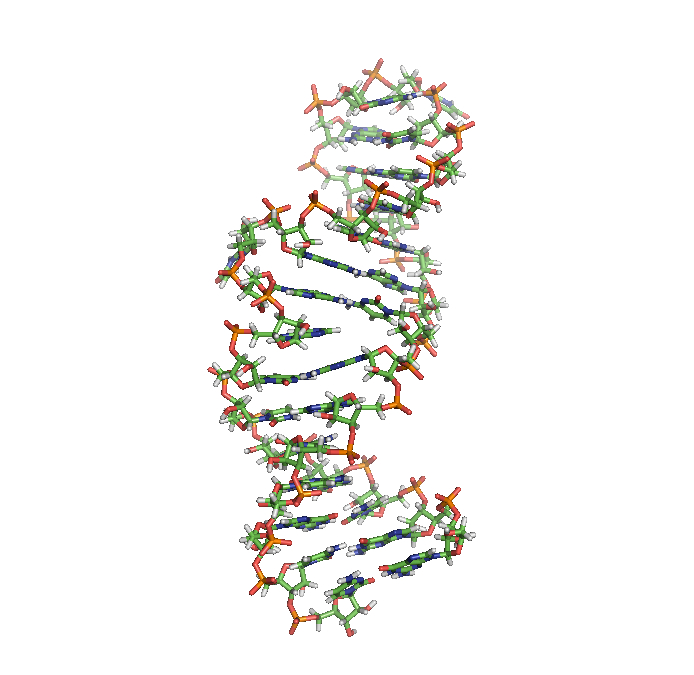
\includegraphics[width=0.6\textwidth]{1KP7}   
      \caption{The internal loop HCV IRES IIIb CA variant of the
        Hepatatis C virus}
      \label{}
\end{figure}

The hepatitis C virus (HCV) internal ribosome entry site (IRES) is
recognized specifically by the small ribosomal subunit and eukaryotic
initiation factor 3 (eIF3) before viral translation initiation.  This
makes it a good candidate for new drugs targetting Hepatatis-C virus.
Our aim is to use REMD to enhance our sampling of the conformational
flexibility of internal loop referred to as {\it HCV IRES IIIb CA
  variant}~\citep{Collier:2002wd} as well as the equilibrium
energetics.  The model used for this work comprises of a 30
nucleotides RNA, and the total number of atoms in the simulating box
is 21887 -- includes the RNA system, explicit water molecules, and
ions for neutralization of the system.  The initial conformation of
the RNA is taken from the NMR structure (PDB ID: 1PK7).  


% However, even with the most powerful computing resources
% at the moment, straightforward MD simulations are unable to reach
% the relevant time-scales required to study conformational changes
% and searches. This is partly due to the inherent limitations in the
% MD algorithm -- a global synchronization is required at the end of
% each time step. 

% RE simulations can be thought of as consisting of two distinct
% components: the underlying simulation engine used for each replica,
% and the coupling-mechanism between the individual replicas. 

% It is important to note that RE is in fact a class of algorithms and
% not a specific algorithm;% ~\citep{dpa-paper}
% for example, different simulation strategies -- Monte Carlo or MD --
% can be used, as well as multiple levels-of-coupling.

\alnote{I think this section could go and be replaced with a
  description of the real science problem.}  


% The degree and frequency of coupling and exchange can be either
% regular~\citep{hansmann,Sugita:1999rm}, or
% irregular~\citep{PhysRevLett.86.4983,pande_bj03}. An example of the
% latter -- parallel replica dynamics as implemented in Folding@home
% \citep{folding} involves coordination between replicas only when an
% ``event'' occurs.  In contrast, for regular RE applications, attempts
% to exchange states between certain pairs occur at fixed intervals. A
% major challenge common to both types is the design, development and
% deployment of a general purpose RE framework for distributed
% environments.

% The framework presented in this paper is used to study possible
% drugs for the Hepatitis C virus. 

\alnote{NEED TO PUT SOMEWHERE: It is noted that the size of the model
  is challenging for conventional REMD, and thus with our framework,
  several interesting outcomes are expected in addition to
  significances of investigation on biological process relevant to
  this RNA system. They are 1) limitation of conventional REMD 2)
  usefulness of other advanced techniques for overcoming the size
  problem such as hybrid REMD, REMD with the solute tempering, and
  many 3) optimization conditions with respect to both implementations
  of our distributed REMD framework as well as REMD algorithms
  associated with exchange efficiency and convergence efficiency.  }

\section{Implementing Distributed Replica-Exchange Using SAGA/Migol}
\label{sec:remd_impl}

\jhanote{Create ``subsections'' using inline beginnings}

\jhanote{Correct/removed references to Old Figure 1}

{\it \bf RE-Manager Architecture:} The
framework comprises of three components, the RE-Man\-ag\-er,
the Replica-Agent and the Migol infrastructure. 
The  \emph{RE-Manager}, also referred to as task manager,
is deployed on the user's desktop and provides the user interface 
to the overall RE run. It orchestrates all replicas, i.\,e.\ the 
parameterization of replica  tasks, file staging, job spawning 
and the conduction of the RE itself using the SAGA APIs.                                                                

The second element is the task agent, the \textit{Replica-Agent},
that resides on the high performance machines where RE simulations
are carried out. The \replicaagent\ is launched using SAGA-CPR and Migol.
%It is responsible for spawning and monitoring of the replicas. 
NAMD~\citep{Phillips:2005gd}, a highly scalable, parallel MD code, is
used to carry out the MD simulation corresponding to each replica
run. It is important to mention that any other MD or
Monte Carlo code could be used just as simply and effectively.
Finally, Migol handles the reliable execution of replicas, i.\,e.\ the
submission, the monitoring and, if required, the recovery of replicas
or the application itself.

% The last component is Migol and the underlying Globus middleware.



\jhanote{This part currently conflates architecture and control-flow}
                       
\noindent                                            
{\it \bf Replica-Exchange Logic:} RE simulations involve the running of multiple replica jobs to enhance
the sampling of configuration space. In the case of REMD each replica
job is assigned a different temperature.  Depending on the number of
configured processes $n$, the \remanager\ creates $\frac{n}{2}$ pairs
of replicas.  Before launching a job the \remanager\ ensures that all
required input files are transferred to the respective resource. For
this purpose, the SAGA File API and the GridFTP adaptor are used.  
The replica jobs are then submitted to the resource using the SAGA-CPR API and
Migol/GRAM. 

When all replicas reach a pre-determined state (e.\,g., the NAMD job
finishes after a fixed number of steps), the decision as to whether to
pairwise exchange temperatures between neighbouring replicas is
determined by the Metropolis scheme. %~\citep{metropolis:1087}.  
The state between exchanges -- that is, the run of an ensemble of replicas
in parallel and the subsequent attempt to pairwise exchange all the
replicas, is referred to as generation. No two replicas can belong to
different generations.  If successful, parameters such as the
temperature, are swapped. Both jobs are then relaunched using the
mechanisms described above. Often the Metropolis scheme returns a
negative result, and an exchange is not carried out; thus it is
difficult to respond to a possible exchange speculatively.

\alnote{Should we make this a subsection or a section? In my opinion,
the GlideIn stuff is a major contribution of this paper -- thus I decided to
give it a separate section. I also think it is more readable than going to the
subsubsection level.}           
         
\noindent
{\it \bf Deploying on Production Environments:} The RE framework has 
been successfully deployed on production
environments, such as LONI and the TeraGrid~\citep{Luckow:2008la}.
The RE-Manager, must periodically obtain the results of all replicas
to determine the new configurations for the next generation.  As the
number of replicas increases, the probability of an overall slowdown
caused by the synchronization after each
generation increases.  A major reason for such a slowdown is the fact that
re-started replicas are required to queue again at
the local scheduler.  In pathological cases, the complete system can
come to a halt caused by a single crowded or slow resource.

To avoid such bottlenecks, the multiple sub-tasks that comprise
distributed applications need to avoid re-queuing at the system
batch-queue level.  Additionally, distributed applications that are
decomposable into sub-tasks should be able to respond to the dynamic
availability of resources.  Unfortunately, current infrastructure does
not support such dynamic scheduling directly, thus in order to provide
this capability to applications we need (i) abstractions that enable
agile execution models via application-level allocation of resources,
and (ii) different adaptivity strategies that determine how resources
are efficiently utilised.  {\it The following section describes the
  extensions to the simple RE framework that enables efficient
  scheduling of sub-tasks and supports adaptive applications.}




% which allows the simple clustering of tasks
\jhanote{Do you see the important difference: BigJob is the clustering
  of tasks; Glide-In is the scheduling mechanism that utilises it to
  solve the repetitive queuing problem}

\alnote{removed Glide-In introduction and move it to next
  section... Otherwise too much redundancy}
\vspace{-0.15in}
\section{Adaptive Replica-Exchange: Abstractions and Implementation}
\label{sec:glidein}
\jhanote{Inlining needs to be used to save space}

As motivated before, the use of multiple {\it simple} Grid jobs to
execute many replicas has a severe limitation: all simple jobs must
queue at the resource management system, i.\,e.\ a single delayed
job can cause an overall slowdown.  We overcome
this issue by using an efficient dispatching scheme, which builds upon
the ability to cluster replicas using the novel BigJob abstraction
before submission. Based on this abstraction, we propose different
strategies that address the dynamic conditions of distributed
environments.

\alnote{Made a minor correction. Adjusted to new structure of section
  5. I am not sure whether there is too much redundancy to 4b}

\alnote{Structure: 1) Intro to cluster job sub, bigjob, glide-in 2.)
  formalism Thus, I commented this out: In this section we provide
  details of our implementation, but before that we will discuss some
  simple formalism so as to understand the terms and establish
  connections to other work better.  }

\alnote{How do we align enhanced job model and BigJob abstraction?}

\jhanote{Enhanced job model is SAGA specific; BigJob isn't. Also one
  is a ``model'', whilst the BigJob is with a specific application
  need in mind. Thus in addition the truth is there are levels of
  abstractions, it what is an abstraction and what is a model is a
  matter of perspective/origin too}              

%{\it \bf Patterns and Abstractions:}  To understand the relationship
% between clustered job submissions, BigJob and Gli\-de-Ins, it is
% useful to review two basic underlying concepts, \I{patterns} and
% \I{abstractions}.  \alnote{I commented this out (liked the second
%   definition of pattern better): A pattern is a references to a
%   commonly occurring mode -- whether in programming an application, in
%   the way an application is used or executed.}  \I{Patterns} are the
% formalization of frequently reoccurring modes, either in programming
% an application or in the way an application is used or executed.  For
% example, the need to submit multiple jobs together is a common
% requirement and practice, and thus provides a simple example of an
% execution pattern.

% A mechanism that supports a pattern is referred to as an
% \I{abstraction}; just as patterns can be programmatic or execution, so
% can abstractions.  \jhanote{Should we give another example, rather
%   than the clustered-job pattern? AndreL, AndreM: any suggestions?}
% \alnote{I think 1 example is supporting our use case is sufficient.}
% For example, 
{\noindent \it \bf Abstractions:} There exists a commonly employed approach to
avoid queuing delays through the use of place-holder jobs, which is
able to dispatch several sub-jobs without each sub-job needing to
queue at the local scheduler. A specific mechanism to support this
pattern is the \emph{Glide-In} abstraction, in reference to the Condor
Glide-In system~\citep{citeulike:291860}, which pioneered this idea. A
Glide-In job requests a sufficiently large chunk of resources; smaller
sub-jobs can then rapidly be executed through the Glide-In job.  By
avoiding the high initial costs for queueing each individual replica
job, the time-to-completion can be dramatically reduced.

% \begin{figure}[t]
%       \centering
%       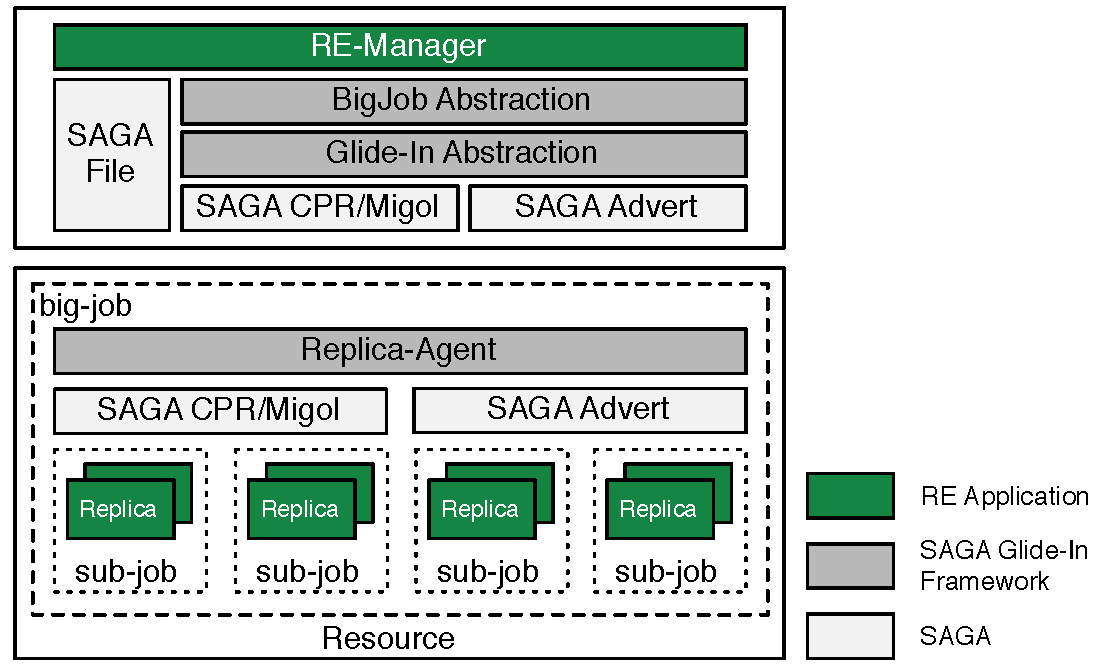
\includegraphics[width=0.7\textwidth]{remdmanager_v12}   
%       \caption{\footnotesize \bf RE-Manager Abstractions: The BigJob
%         abstraction provides the capability to cluster sub-jobs into a
%         larger big-job, and is implemented on top of the Glide-In
%         abstraction.}
%       \label{fig:abstractions}
% \end{figure}

% \begin{figure}[t]
%   \centering
%       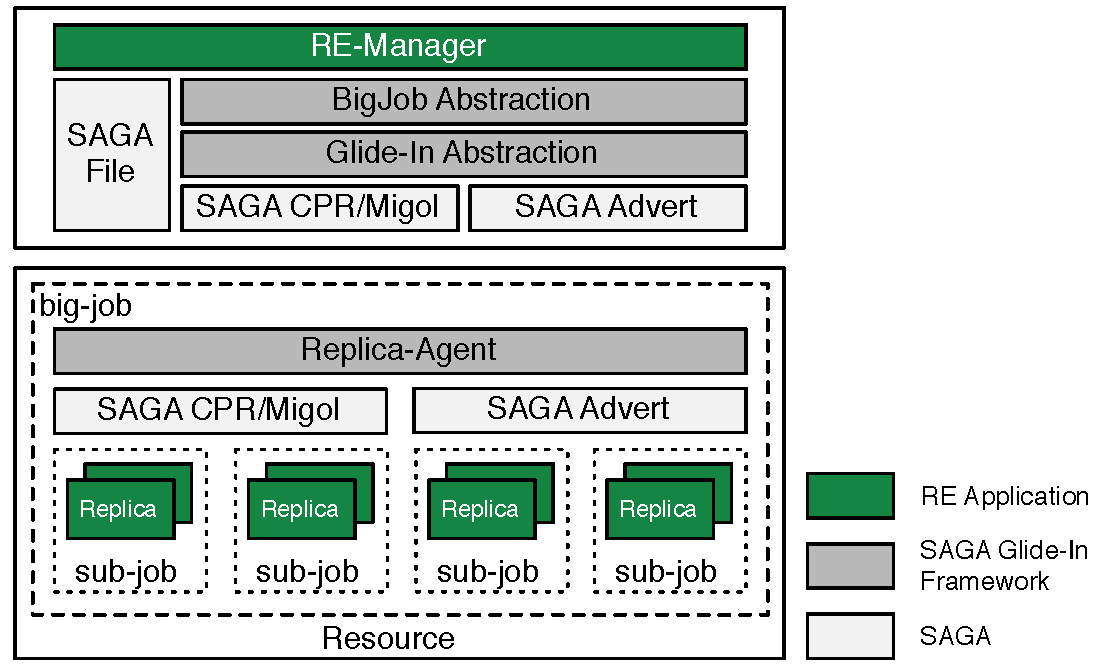
\includegraphics[width=0.7\textwidth]{remdmanager_v12}   
%       \caption{\footnotesize \bf RE-Manager Abstractions: The BigJob
%         abstraction provides the capability to cluster sub-jobs into a
%         larger big-job, and is implemented on top of the Glide-In
%         abstraction.\vspace*{-3em}}
%       \label{fig:abstractions}
% \end{figure}
% 
% \begin{figure}[t]
%     \centering
%     % 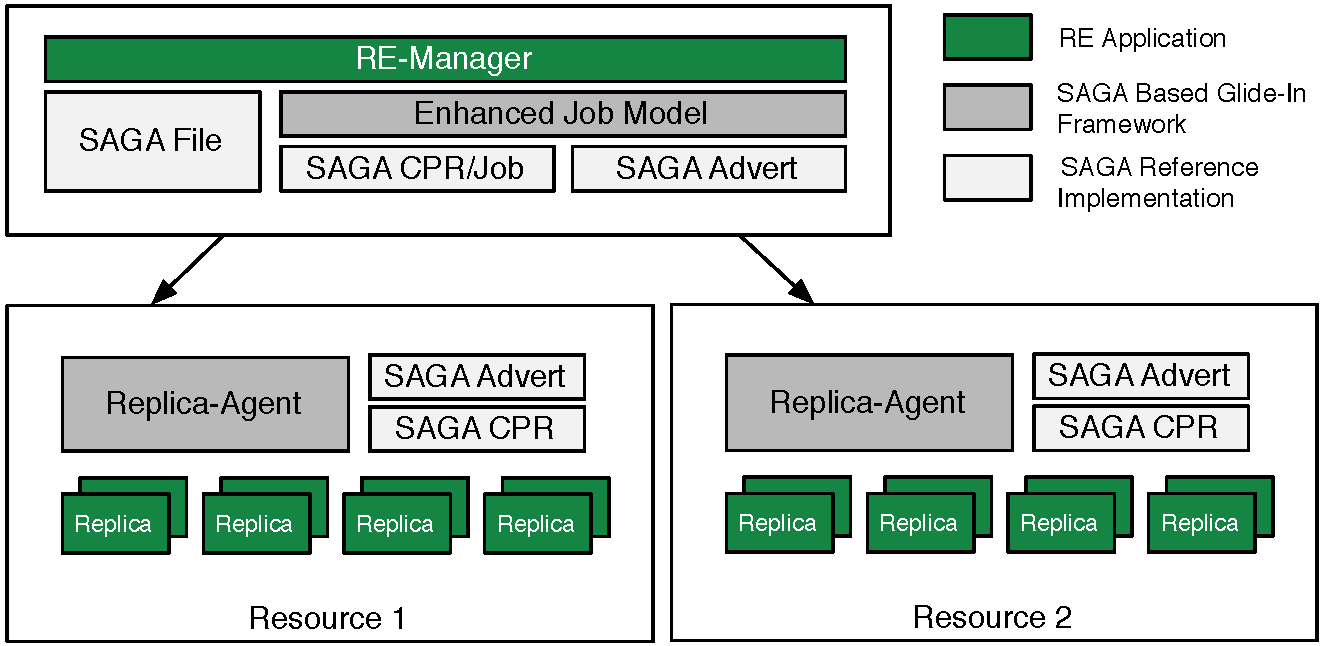
\includegraphics[width=0.9\textwidth]{remdmanager_v11}   
%     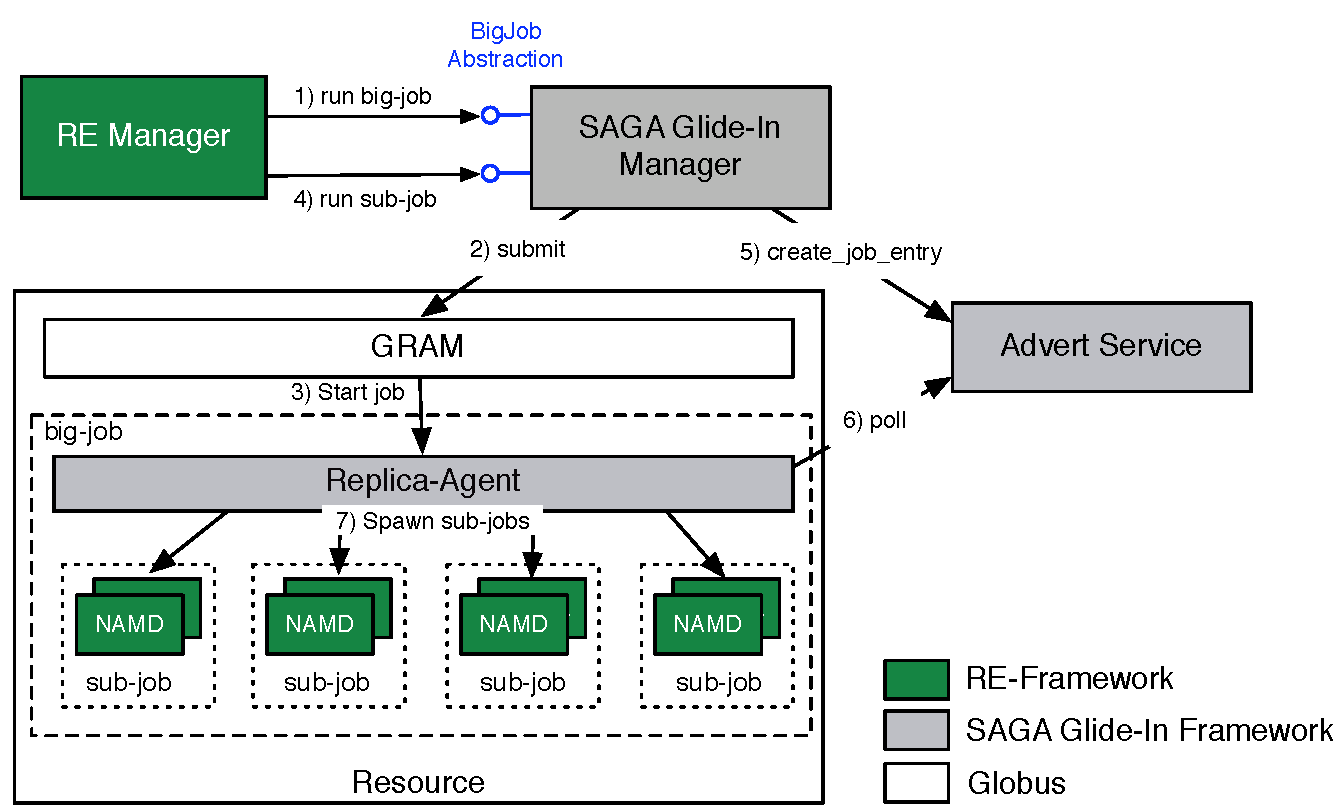
\includegraphics[width=0.7\textwidth]{re_bigjob_interactions}   
%     \caption{\footnotesize \bf RE-Manager and SAGA-Glide-In Framework:
%       The Glide-In job (\replicaagent\ ) is used as place-holder job
%       for all replica sub-jobs running on a single cluster. The
%       \remanager\ can control both the \replicaagent\ and the replica
%       jobs. % Glide-In provides an effective way to provide resources
% %       to the application directly and not to the sub-jobs.
%     }
%     \label{fig:remdmanager_v1.1}
% \end{figure} 
                      
\begin{figure}[t]
  \begin{minipage}[t]{.47\textwidth}
    \begin{center}  
      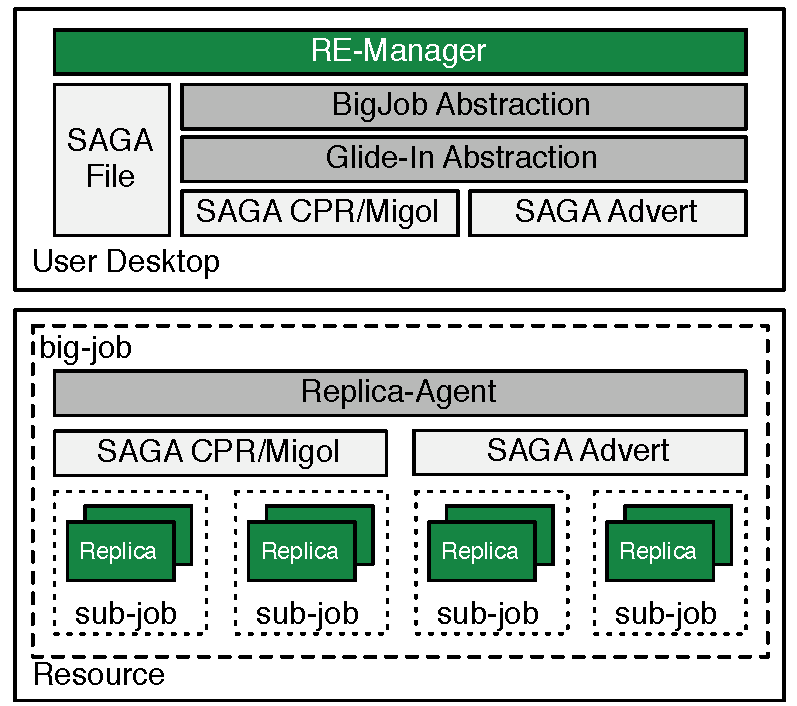
\includegraphics[width=0.9\textwidth]{remdmanager_v13}
      \caption{\footnotesize \bf RE-Manager Abstractions: The BigJob
          abstraction provides the capability to cluster sub-jobs into a
          larger big-job, and is implemented on top of the Glide-In
          abstraction.\vspace*{-3em}}
     \label{fig:abstractions} 
    \end{center}
  \end{minipage}
  \hfill
  \begin{minipage}[t]{.51\textwidth}
    \begin{center}  
     
%      This scenario utilises the capability of the underlying physics
%      model to
      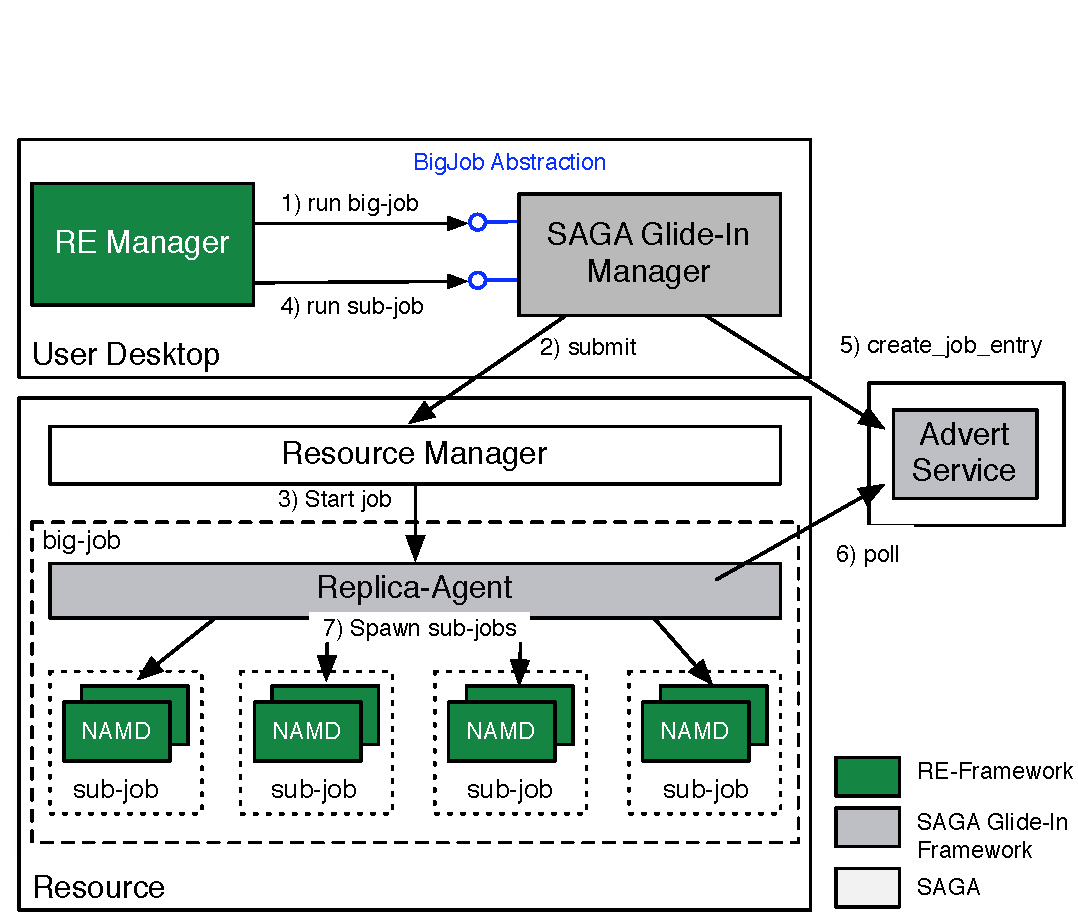
\includegraphics[width=\textwidth]{re_bigjob_interactions_v2}
      \caption{\footnotesize \bf RE-Manager and SAGA-Glide-In Framework:
        The Glide-In job (\replicaagent\ ) is used as place-holder job
        for all replica sub-jobs running on a single cluster. The
        \remanager\ can control both the \replicaagent\ and the replica
        jobs.}
        \label{fig:remdmanager_v1.1}   
    \end{center}
  \end{minipage}
  \hfill
\end{figure}



% \begin{figure}[!h]
%   \begin{center}
%     \subfigure{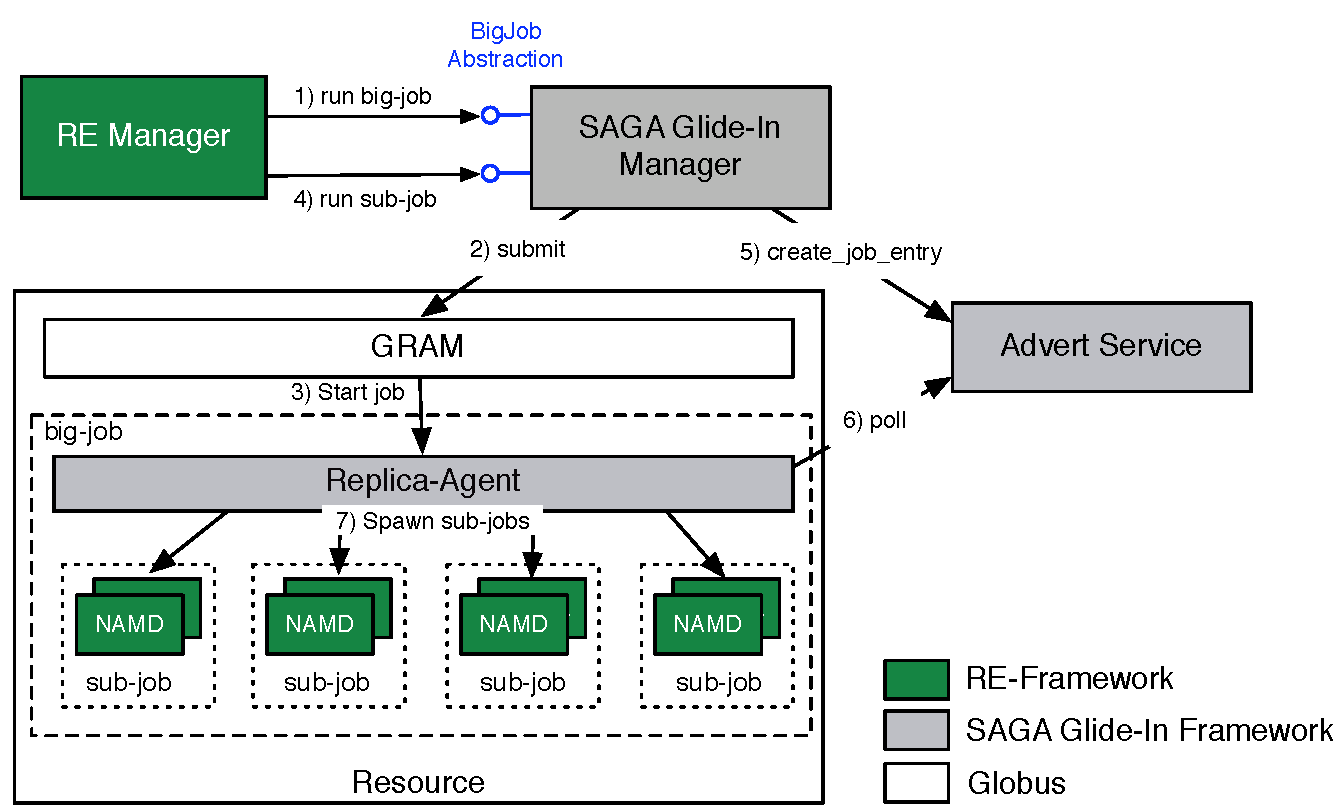
\includegraphics[width=3.5in]{re_bigjob_interactions}}
%     \subfigure{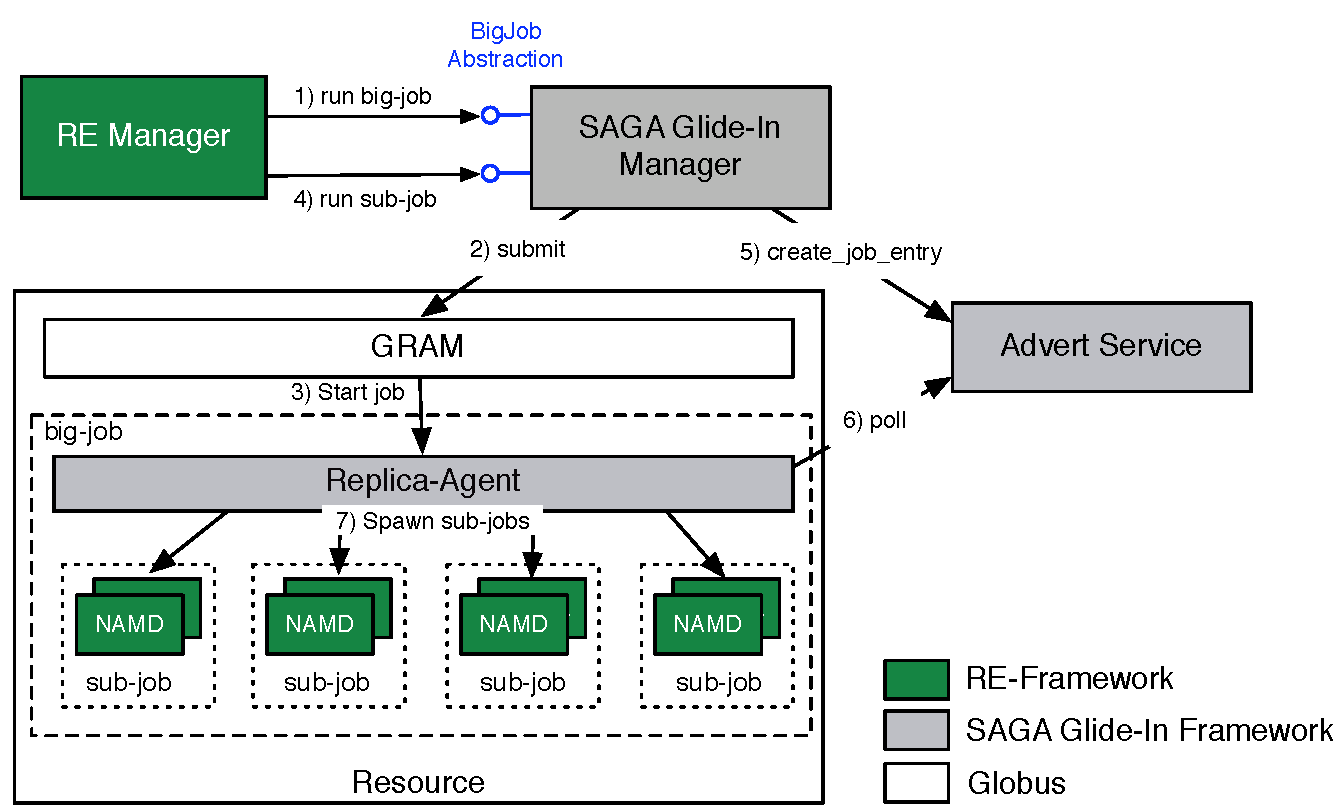
\includegraphics[width=3.5in]{re_bigjob_interactions}}
% }
    

% , which implements a place-holder job for effective scheduling.
% SAGA Glide-In is implemented using capabilities provided by SAGA --
% in particular SAGA-CPR and Advert.

Figure~\ref{fig:abstractions} summarizes the abstractions developed
and used in this work to support the clustering of sub-jobs into a
larger big-jobs and the effective dispatching of the sub-jobs.  The
specific capability to cluster sub-jobs, is provided to the
application via the \emph{BigJob} abstraction. 
% This abstraction
% enhances the SAGA job model \jhanote{Need a sentence or two about what
%   ``enhancing the SAGA job model'' means, ie in turn outlining what
%   the SAGA Job Model is?}  with the capability to allocate
% larger chunks of resources for an applications, which can then be used by 
% multiple sub-jobs.
% \jhanote{AndreL: Not sure what the commented out line was about.. if
%   you'd like to reinstate, please clarify/elaborate}
Another abstraction -- the SAGA Glide-In abstraction is used to
support the commonly occurring requirement to schedule multiple
sub-tasks relative to each other and not in competition with other
jobs submitted to the batch queue system.  Thus, a \texttt{big\_job}
and \texttt{sub\_job} object are defined; for each \texttt{big\_job}
object, a Glide-In job with the desired number of resources is
started, and \texttt{sub\_job} objects -- which correspond to
individual replicas, are mapped to a \texttt{big\_job} using the jobid
as reference. It is helpful to reiterate that although there is a
big\_job object, it is submitted as a Glide-In job, and that BigJob
abstraction in turn utilises the Glide-In abstraction to map the
individual big-job and sub-jobs to physical resources.

% \begin{figure}[t]
%     \centering
%     % 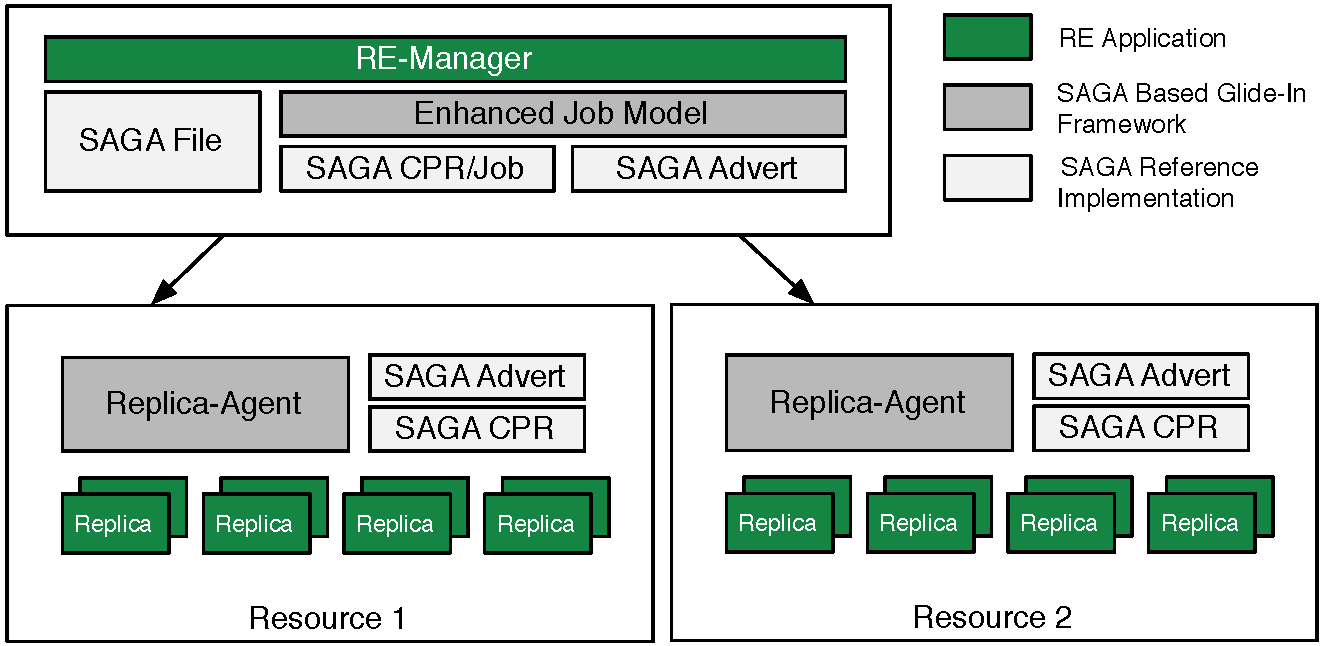
\includegraphics[width=0.9\textwidth]{remdmanager_v11}   
%     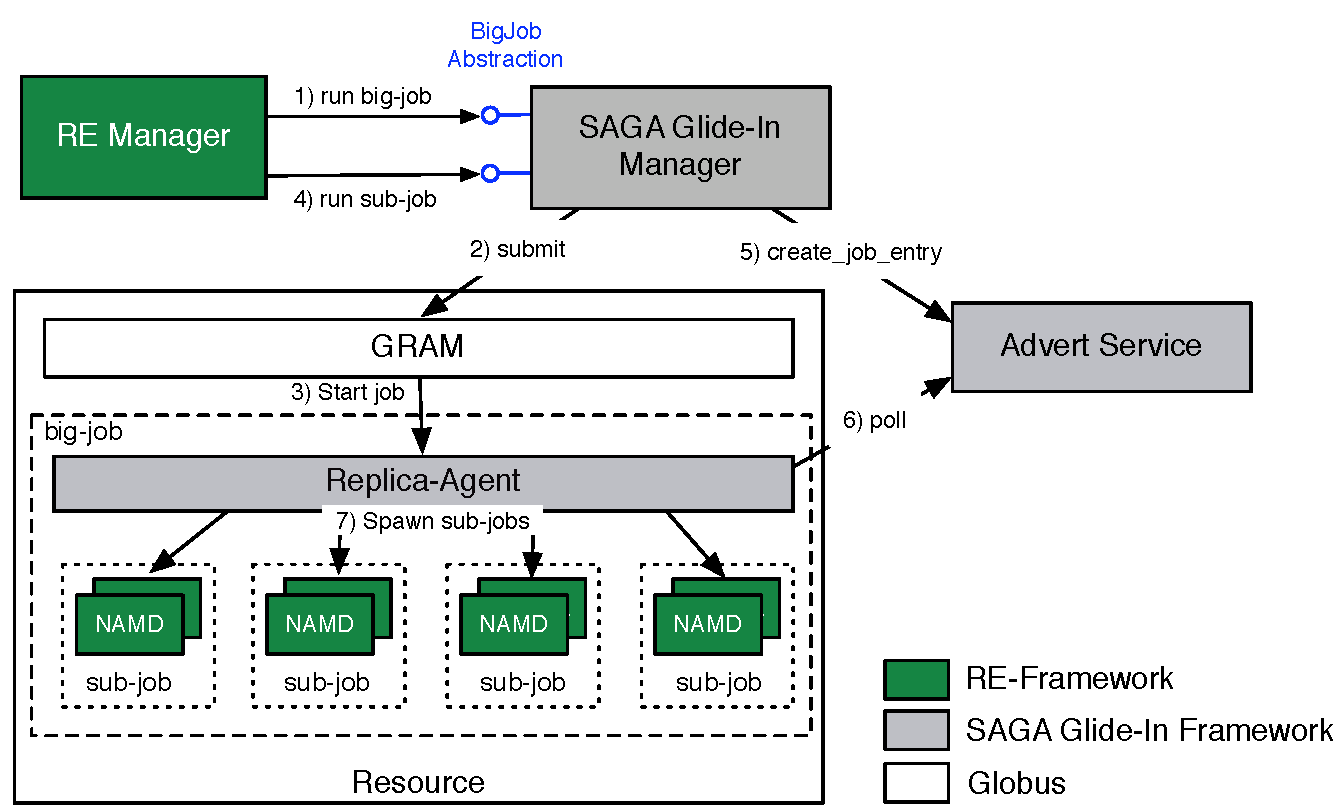
\includegraphics[width=0.7\textwidth]{re_bigjob_interactions}   
%     \caption{\footnotesize \bf RE-Manager and SAGA-Glide-In Framework:
%       The Glide-In job (\replicaagent\ ) is used as place-holder job
%       for all replica sub-jobs running on a single cluster. The
%       \remanager\ can control both the \replicaagent\ and the replica
%       jobs. % Glide-In provides an effective way to provide resources
% %       to the application directly and not to the sub-jobs.
%     }
%     \label{fig:remdmanager_v1.1}
% \end{figure}
    
%using a SAGA-based user-level job API (the BigJob
      %abstraction).
%  are minimized and the time-to-completion can be
%       dramatically reduced.
% RE-Manager overall
{\noindent \it \bf Implementation:} The RE framework presented in section~\ref{sec:remd_impl} has been
extended to support the management and scheduling of replica jobs.
BigJob provides the ability to cluster sub-jobs; Glide-In provides the
ability to effectively schedule the sub-jobs.  As illustrated in
Figure~\ref{fig:remdmanager_v1.1}, the RE-Manager uses the
\texttt{big\_job} and \texttt{sub\_job} objects as replacement for the
\texttt{job} object defined by SAGA CPR.  The \texttt{big\_job} and
\texttt{sub\_job} objects behave similarly to regular SAGA CPR job
objects. Thus the RE-Manager, which is the application in this case,
does not require any extensive modification to accommodate this
replacement; all that the RE-Manager has to do additionally, is
provide a mapping from a \texttt{sub\_job} to a suitable
\texttt{big\_job} via a jobid.

% BigJob
The SAGA Glide-In implementation comprises of three components: 1) The
\emph{Glide-In Manager}, which as the name suggests manages the
orchestration and scheduling of Glide-In jobs (which in turn allows
the management of both big-job objects and sub-jobs) and 2) The
\emph{Replica-Agent}, which represents the Glide-In job and thus, the
application-level resource manager on the respective resource, and 3)
the \emph{Advert Service}, which is used for communication between the
Glide-In Manager and Replica Agent.


Before running regular jobs, an application, in this case the 
RE-Manager, must initializes a
\texttt{big\_job} object. The Glide-In Manager then queues a Glide-In
job, which actually runs a Replica-Agent on the respective resource,
using the SAGA-CPR API.  For this \texttt{big\_job} instance the
specified number of resources is requested. Subsequently,
\texttt{sub\_job} objects can be submitted through the Glide-In
Manager using the jobid of the \texttt{big\_job} as reference.
The Glide-In Manager ensures that the sub-jobs are launched onto the 
correct resource based upon the specified jobid using the right number
of processes.

Communication between the Replica-Agent and Glide-In Manager is
carried out using the SAGA Advert Service, a central key/value
store. For each new job an advert entry is created by the
RE-Manager. The \replicaagent\ periodically polls for new jobs.  If a
new job is found and resources are available, the job is directly
dispatched, otherwise it is queued. Further, the agent encapsulates
local machine-specific settings. The \replicaagent\
ensures e.\,g.\ that the right combination of compiler, MPI library and NAMD
executable is used.


\jhanote{``The enhanced job used by the BigJob abstraction can be used
  as drop-in replacement for a SAGA job object.'' The previous line in
  quotes, is confusing. BigJob is an abstraction, and big-job is
  implementation. Let us not address enhanced job model in the
  implementation section; remember it is a SAGA specific thing}

\alnote{I think this is redundant to the first paragraph: As 
shown in Figure~\ref{fig:remdmanager_v1.1}, a big-job object is
submitted to the SAGA Glide-In Manager, which queues a Glide-In job
onto a specific resource. Then when sub-jobs are submitted by the
RE-Manager, they are launched onto the correct resource based upon the
job id, and with the right number of processors.  }

\label{sec:adaptivitiy}    
\alnote{Is this a worth a new section or does it rather belong to
  5b). We should probably join both sections.}  

\jhanote{Sorry, if I missed answering this Q earlier, but yes, I think
  if there is a way of merging the two sections, then that will be
  good. Something along the lines of, ``Abstractions to Support
  Adaptive Replica Exchange'' or ``Abstractions to Support Adaptive
  Replica Exchange: BigJob and SAGA Glide-In''}

\alnote{I shrinked this section pretty much... Maybe the some more
    aspects from the original section could be added. The complete
    section is commented out below.}

  {\noindent \it \bf Adaptive Replica Scheduling:} Distributed applications
  including RE simulations must be able to deal with time-varying
  resource availabilities.  An application is referred to as
  \emph{dynamic} when either the resource requirements of the
  application, or the availability and utilisation of resources by the
  application changes during its runtime.  \emph{Adaptivity} is a
  mechanism to respond to dynamic
  changes; % as opposed to just ignoring the dynamism of a distributedenvironment.
  a dynamic application may deploy multiple adaptive strategies or
  choose between competing adaptive strategies.  For an application to
  be adaptive, it is necessary for it to be able to effectively
  utilise an expanded or reduced set of resources; additionally for an
  adaptive application to be scalable it must also be able to
  determine which resources to utilise efficiently, if not optimally.
  For resource determination, our framework currently relies on a
  static, user-defined mapping of replicas and resources.  In the
  remainder of this paper, we will focus on dynamic resource
  utilisation (and not on dynamic resource determination or
  optimisation).

For jobs that want to maximise their throughput the ability to adapt
to dynamically changing resource loads and requirements is
critical. It is equally important for long-running applications to be
able to support an agile execution model allowing the effective
utilisation of resources as they become available.  Specifically,
there are different ways a RE simulation can respond to a change in
the number of resources required/available:
\begin{compactitem}         
\item {\it Scenario A:} By increasing the number of processes assigned
  to replicas the time-to-completion can be reduced. In addition,
  resources can be partitioned in a way that balances the different
  speeds of resources.  For example, by adding processes to a 
  delayed replica, bottlenecks due to synchronisation of replicas can
  be avoided.
  %light-coupling between all replicas can be avoided.
  \jhanote{AndreL: The last sentence needs more elaboration before it
    makes sense. Plus slowdown maybe due to heterogenous resources,
    but in some cases, it could be due to late start, especially if
    exchange takes place between replicas on different machines}
  \alnote{Ok, I elaborated the last sentence a little more. One more
    remark: when using SAGA Glide-In the late start effect should not
    exist.}

\item {\it Scenario B:} As resources become dynamically available, the
  number of replicas can be adjusted. Depending on the underlying
  physics model, the additional replicas can be used to either refine
  the temperature range (adaptive sampling) or to extend the
  temperature range (enhanced dynamics).
\end{compactitem}           
% Both adaptive strategies have been realized within the RE-Manager, and
% BigJob and Glide-In are useful abstractions in both scenarios. 
Our framework supports both adaptive strategies.

% Our framework supports and implements both strategies.  

\jhanote{We need a better place for this paragraph. It is an important
  paragraph, but probably not well suited here -- where the discussion
  is all about adaptivity. The paragraph below is about
  agile-execution supporting adaptivity while there is no mention of
  adaptivity and MPIg jobs.}
\alnote{I commented this paragraph about MPIg out. Most of the points are
made in related work (work of owain). We could also extend the criticism
there, but I am not sure about the politics thing...}  

\jhanote{Difference between schema and scheme!}
\alnote{ok got it, scheme is more suitable in most cases when referring to adaptive
scheduling scheme}
\jhanote{This is a dangerous remark to
  make. Not sure if I wrote it in the first place, or AndreL did, but
  either way, it has to be either substantiated or removed. We can
  argue qualitatively that we maybe be better, but the last sentence
  is a Quantitative remark and that is unacceptable without data to
  back it up. Thoughts?}

\jhanote{We could caveat it by saying, short-running or remind the
  reader that is the only way for systems that do not provide
  co-scheduling of resources}

\alnote{I tried to rephrase this sentence a little. I think for loosely coupled
apps, co-scheduling is less relevant than for coupled apps. However,
we did not do a performance study... Thus no data.}   

\jhanote{Secondly, it is important to distinguish between the new
  ``Job abstraction'' ie meta-job and simple-job as an extension of
  the SAGA job-model, from the \glidein\ abstraction. I am sure we are
  all aware of the differences, but in the writing the two seem to be
  conflated, or at least will appear conflated for a person reading
  this the first time. I would say the mata-job/simple-job is a usage
  pattern, and the \glidein\ is an abstraction that supports this
  pattern.}

\jhanote{We could probably structure the subsection on ``Efficient
  Replica Job Scheduling'' into two parts, an opening on ``Job
  Patterns and Abstractions'' and secondly
  ``Implementations''. Currently, we need more details describing
  Figure 2 and the control flow between \remanager\ and individual
  replica-jobs within a meta-job. This location of this note, is a
  good point to separate the two.}    


\section{Distributed Replica-Exchange on the TeraGrid}
\label{sec:exp}
        
To evaluate the performance of the RE-Manager several experiments have
been conducted on the TeraGrid (TG) and LONI resources. The resources
used are: Ranger (TG), Abe (TG) and QueenBee (QB; both TG and LONI).
% We investigated the performance of the SAGA Glide-In mechanism under
% different adaptivity modes.  
The RE-Manager was configured to run a MD simulation with up to 16
replicas sampling a temperature range between 300 and 450\,K. Replica
exchanges are carried out between pairs of replica processes, thus
there are up to 8 exchanges in each generation; each test run comprises
of up to 64 attempted exchanges\jhanote{AndreL: I don't think the
  numbers add up here!}  \alnote{Yes, they do not add up. I
  standardized all figures to T\_c for 64 attempted exchanges} Each
replica is a parallel NAMD simulation, can use up to 24 MPI processes
and runs for 500 time steps between exchange attempts. The metric of
performance used in our tests, is the time-to-completion for 64
attempted exchanges.

\jhanote{the use of the term cluster should be consistent with the
  resource description :)}

\jhanote{define Generation?}  \alnote{added definition to introduction
  - should we define it here also?}  \jhanote{distinguish between
  replica, replica processes; or at least keep usage consistent}
\alnote{OK, hopefully use replica consistently} \jhanote{describe how
  exchange partner is chosen? remains the same?}\alnote{yes, the pairs
  remain the same. Added a sentence.}


\jhanote{unfortunately this paragraph and the one before are unclear}
\jhanote{I would recommend using time-to-completion over
  time-to-solution; also maybe use shorthand T\_c?}  \jhanote{Ah, OK
  single-machine is mentioned here now. Need to mention explicitly
  upfront} \alnote{hopefully mentioned sufficiently often now}

Initially we investigated the effect of the SAGA
Glide-In framework on the time-to-completion ($T_{c}$) using 16
replicas on QB.  Using the Glide-In framework, there was a reduction
in $T_{c}$ from 52\,minutes to about 26 minutes per average, which
corresponds to a decrease of about 50\,\% runtime.  In the best case,
improvements of up to 70\,\% were observed. As described, this effect
is mainly attributed to the elimination of queuing times for every
sub-job. Once the Replica-Agent becomes active, replicas can be
efficiently dispatched without requiring interactions with the local
scheduler.

\jhanote{need to clarify what the 80\% means/implies?} \alnote{I
  refined the above paragraph. Are there any particular implications
  you refer to?}

\jhanote{We need to say something about the location of the kink when
  glide-in is not used. This is another way of addressing the erratic
  behaviour. Do we have insight as to whether the kink often occurs
  sooner than at 8 replicas? If so, how often.  This would help us
  reiterate that the use of glide-in gives a constant/static
  performance estimate, whereas the lack of a GlideIn makes it
  erratic.}  \alnote{I updated the data. This were still the old graph
  from MTAGS. I added data from some additional runs, which reduced
  the benefit of Glide-In a little, but also the stdev for the without
  Glide-In case was reduced. Unfortunately, I do not have too many
  data points for the 2, 4, 8 replica processes to really say whether
  there are earlier kinks.  The position of the kink really depends on
  the length of the PBS queue. In this scenario the cluster was not
  too crowded, so that many jobs could be backfilled (but not all jobs
  could be backfilled.)}  \alnote{I describe the slowdown with more
  than 12 replicas above when referring to Fig. 4a. Is this
  sufficient? or should I describe it again down here?}
\jhanote{AndreL: I think this section reads well now. Thanks.}

Further, we performed tests for the two different adaptive scenarios.
In the scenario A, the number of replicas was kept constant and the
\emph{replica size}, i.\,e.\ the number of MPI processes assigned to
each replica (Conventional REMD) was varied.  In scenario B, the
\emph{replica number} -- the number of replicas participating in a
generation was varied. This approach is also referred to as Cool
Walking.  We compare the runtime of the REMD simulation for 64
attempted exchanges on different sets of distributed resources and
Glide-In configurations.
                    
\begin{figure}[h]
  \begin{minipage}[t]{.48\textwidth}
    \begin{center}  
      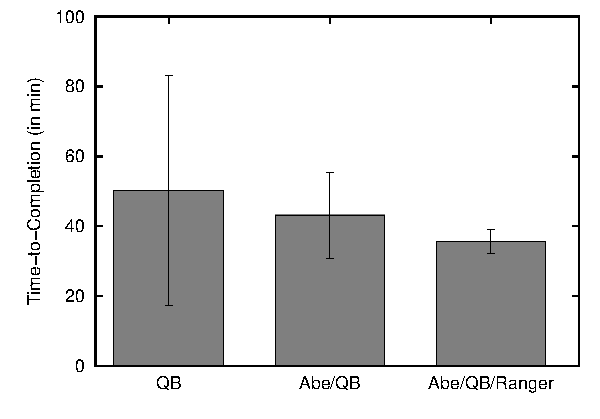
\includegraphics[width=\textwidth]{performance/perf_distributed_size_replica.pdf}
      \caption{\footnotesize \bf Replica Size Adaptivity (Scenario A):
        As the number of resources available increases, the number of
        cores assigned to a replica (a NAMD job) is dynamically
        adjusted, while keeping the number of replicas constant at
        sixteen.  There are 4~Glide-Ins, and each has 32 core assigned
        to it.  As more resources become available, more cores can be
        assigned to each replica (NAMD job) which leads to a reduction
        of $T_{c}$.  }
      \label{fig:performance_perf_distributed_A}
    \end{center}
  \end{minipage}
  \hfill
  \begin{minipage}[t]{.485\textwidth}
    \begin{center}  
     
%      This scenario utilises the capability of the underlying physics
%      model to
      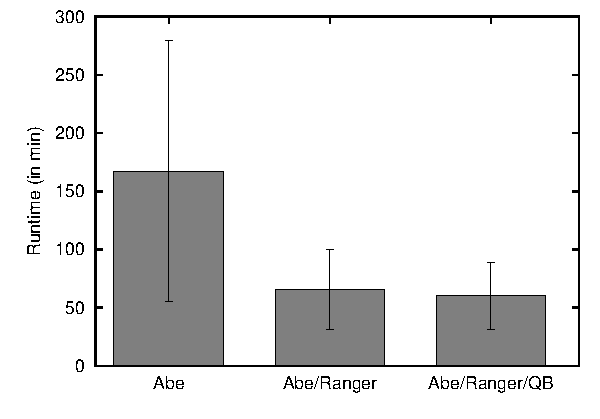
\includegraphics[width=\textwidth]{performance/perf_distributed_number_replica.pdf}
      \caption{\footnotesize \bf Replica Number Adaptivity (Scenario
        B): In this scenario, the framework dynamically adjusts the
        number of replicas.  A constant number of 4 Glide-Ins with 64
        cores each are distributed across 1, 2 and 3 machines; the
        size of each replica is kept fixed at 16 cores. Once again,
        the greater the number of distributed resources that can be
        utilised, the smaller $T_{c}$.}
      \label{fig:performance_perf_distributed_B}
    \end{center}
  \end{minipage}
  \hfill
\end{figure}

In scenario A, up to 3 different resources are used, the number of
Glide-Ins varies from 4 upto 12, whilst the number of replicas used is
fixed at 16. Thus, the size of the individual replicas is varied.
When a resource is being used, it runs 4 Glide-Ins and each Glide-In
job has a constant size of 32 cores each.  Although, the number of
Glide-In jobs on a resource is fixed at 4 for reasons of simplicity,
our results will hold for general values of this parameter. If all
resources (Abe, QB and Ranger) were being used, there would be 12
Glide-In jobs with 32 cores each, for a total of 384 cores.  Glide-Ins
are submitted to one, 2 or 3 statically configured resources. Usually,
these Glide-Ins are subject to different queueing delays at the local
scheduler. To reflect these different resource loads, the number of
MPI processes assigned to each of the replicas is dynamically
increased as new resources become available (and therefore the number
of Glide-Ins can be increased). Depending on the number of available
resources, between 8 (for 4 Glide-Ins) and 24 cores (for 12 Glide-Ins)
are used for each replica.

Figure~\ref{fig:performance_perf_distributed_A} shows the results of
the distributed run. In spite of the overhead for migrating replicas
to newly available resources, a notable speedup of up to 15\,minutes
can be observed as the number of resources increases from one to
three. Although, the efficiency, defined as runtime on 1 resource
divided by the runtime on multiple resources scaled by the number of
resources, is only about 0.5, this is a limitation of the used setup
rather than a general scalability barrier.  The setup comprises of
rather short NAMD jobs; in particular during the initial phase jobs
are often migrated to other resources, which mainly causes this
overhead. During longer runs this overhead is essentially
negligible. What is also very important to note is the reduced
fluctuation in the $T_c$ when multiple resources are used. This is
indicative of the fact that there is a reduction in the sensitivity to
queue-loads -- something that applications on real production
environments have to battle with.  \jhanote{AndreL: Mention how many
  times these experiments were repeated? were the three cases repeated
  the same number of times? or was the first case (one machine) done
  more times than the 3 machine run, in which case the error bars are
  even more significant}

\jhanote{I think we need to address
  the following else we will get dinged by the referees: We increase
  our resource pool by a factor of 3, but get only a 33\% improvement
  at best} \alnote{I tried to explain this number a little better
  using the calculated efficiency: (t(1)/t(n))/n: E(2) = 0.58; E(3) =
  0.47; There are still some issues with scenario A (in particular I
  am referring to the heterogeneous speeds of these three machines
  making this increasing number of MPI processes less efficient!)}
\jhanote{I think we should talk about the above remark. Also we should
  define efficiency in the text, else we will get dinged.}  
\alnote{efficiency defined.}

% general setup
In scenario B, the capability of the RE-Manager to adaptively adjust
the number of replicas simulated -- in effect adjusting either the
range of temperature or the specific temperatures simulated, is
evaluated.  For this scenario, 4 Glide-Ins with 64 cores each
are distributed across either 1, 2 or 3 different distributed
resources. That means that the total of 256 cores is allocated on (i)
Abe only, (ii) Abe and Ranger respectively (iii) Abe, Ranger and QB.
Each replica has a constant number of 16 MPI processes, and thus any
Glide-In can run exactly 4 replicas when active.

\jhanote{AndreL: Make it easy for the ready to grasp the number of
  cores used when just Abe; when Abe/Ranger and finally when
  Abe/Ranger/QB. (i) Is it 4 glide-ins in each of the three scenarios?
  4 glide-ins on Abe, then 4 glides-in on Abe/Ranger and then 4
  glide-ins on Abe/QB/Ranger??}

\alnote{Added sentence. Answer to your question: yes}
              
%  procedure
At the beginning of the experiment, all 4 Glide-Ins are submitted to
either 1, 2 or 3 resources (statically configured).  Similar to
scenario A, queueing delays usually occur; this is true whether using
1 resource or using 3.  Consequently, not all Glide-Ins start
simultaneously.  Using the adaptive temperature sampling algorithm,
the number of replicas is dynamically varied as the number of active
Glide-Ins increases. Depending on the number of running Glide-Ins, the
ensemble consists of 4 to 16 replicas (increase in
steps of 4).

\jhanote{I don't understand how the number of replicas can be
  increased if (a) the size of each replica is kept a constant and (b)
  the number of processors assigned remains at 256 in all cases? What
  was the starting value of the number of replicas?}  

\jhanote{Once again, I think we need to put in a few sentences of how
  the experiments were performed. It will help the reader and clear up
  a few things that are difficult to understand.}
% A maximum of 16 replicas and 256 cores are used.

As shown in Figure~\ref{fig:performance_perf_distributed_B}, $T_{c}$
decreases with the number of resources used.  With the the simulation
distributed onto greater number of resources, the probability that a
single heavily-utilised resource delays the overall progress of the
simulation is reduced.
% This is also reflected in the standard deviation,
% which clearly decreases as the number of distributed resources used
% increases. 
The results clearly demonstrate the benefits of the adaptive replica
scheme -- it is favourable to instantly use resources as they become
active instead of waiting for the complete set of nodes to become
available.  

\section{Results: Enhanced Sampling of Hepatitis-C Virus}
In the previous section we discussed the design and performance
of the framework and shown how it enables the effective utilisation of
multiple resources. In Section 2, we described why the RE approach is
required to understand the energetics and conformational flexibility
of the internal loop of the Hepatitis-C virus. The effectiveness of
the RE approach in increasing the rate of convergence to equilibrium
(Boltzmann distribution) or enhancing the sampling can be measured by
the rate of attempted exchanges~\citep{Lei:2007xe}, or equally by the
inverse of the {\it time} between attempted exchanges.

To demonstrate that effectiveness of our RE framework in enhancing
sampling or the rate of convergence to equilibrium for real sized
biomolecular systems, we analyse the typical time-series of resources
used (available) during a six hour run on production infrastructure
(green line in Fig~\ref{fig:result_A}).  REMD simulations (Scenario A)
were performed for HCV IRES IIIb CA variant using the model described
in Section 2. The replicas covered a temperature range from 300 K to
450K, which sets the number of replicas to a fixed value of 16.  Each
glide-in has 32 cpus, and thus the number of cpus for each replica is
determined by the numbers of active glide-in jobs.
Fig.~\ref{fig:result_A} shows how the number of active glide-ins
changed during this six hour interval. To start with, there were only
enough processors to support one glide-in job, but after approximately
two hours, there were enough to support two active glide-ins and three
glide-ins were supported after three hours. Eight glide-ins were
activated before the six hour time limit. As the number of glide-ins
increases, the number of processors assigned to each replica
increases, with the physically important consequence that there is a
concomittant decrease in the average time between exchange
attempts. This is shown in the time-series in red in
Fig.~\ref{fig:result_A}.  The average time between exchange attempts
as a function of the number of active glide-ins is shown in red in
Fig.~\ref{fig:result_B}, whereas the speedup -- measured as the inverse
of the average time normalised by the time taken by one glide-in (thus
the value of 1 for the one glide-in case) is shown green.

\begin{figure}[h]
  \begin{minipage}[t]{.495\textwidth}
    \begin{center}  
      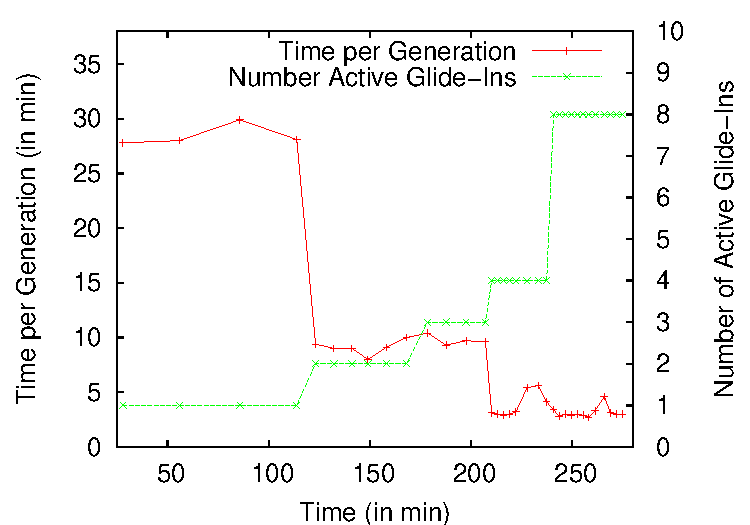
\includegraphics[width=\textwidth]{performance/hepatitis/perf_repex.pdf}
      \caption{\footnotesize \bf Plots showing the time-series of the
        average times between exchange attempts (in red and using the
        left-hand y axis) and the number of active glide-ins over a
        six-hour run on the TeraGrid.}
      \label{fig:result_A}
    \end{center}
  \end{minipage}
  \hfill
  \begin{minipage}[t]{.48\textwidth}
    \begin{center}  
     % \includegraphics[width=\textwidth]{}
      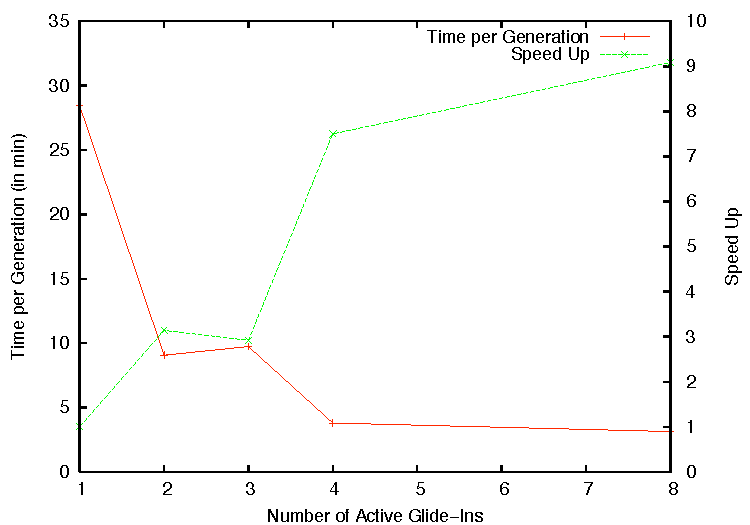
\includegraphics[width=\textwidth]{performance/hepatitis/perf_repex2.pdf}
      \caption{\footnotesize \bf The plot in red (using the left-hand
        y axis) showing how the average time between exchange attempts
        decreases as the number of glide-ins increases. The plot in
        green shows the Speed-up.}
      \label{fig:result_B}
    \end{center}
  \end{minipage}
  \hfill
\end{figure}             


%% ----------------------------------------------------------------------------
\section{Conclusion and Future Work}

\jhanote{Mention BQP and co-scheduling as opposed to opportunistic
  approach. Reference Kalman-filter work. Reference Promita's work
  using BQP for tightly-coupled applications.} 
                
\alnote{I removed some parts due to redundancy}

\alnote{Attempt to structure conclusion: 1) SAGA/Migol 2.) Glide-In
  3.) Adaptive Sampling 4.) Future Work: Glide-In, REMD, Reservation,
  BQP}
                                         
\jhanote{needs smoothening} 

In summary, SAGA provides a well-defined and sufficiently powerful
interface to develop the required abstraction to support adaptive
distributed RE applications.  SAGA also allows the simple decoupling
of the RE orchestration logic from the underlying distributed
infrastructure. The SAGA \glidein\ framework represents the first
known instance of creating a runtime, system-level abstraction for
distributed systems from basic programming interfaces. All this whilst
remaining general purpose and extensible.  The adaptive RE framework
has been successfully deployed on the TG and LONI resources.  Using
the BigJob abstraction, RE sub-jobs could efficiently be dispatched
reducing the time-to-completion up to 70\,\%. The use of different
adaptivity strategies to dynamically utilise additional resources led
to a further reduction of the time-to-completion.

In the future, we will refine our RE framework making it
more adaptive towards dynamic environments, e.\,g.\ by deploying  
a more asynchronous scheme as described by \citet{Gallicchio:2007yq}.
% Further, we will utilise our RE framework to study real science problems,
% such as the Riboswitch problem~\citep{Huang:2008xe}.     
At the same time, we will improve our RE infrastructure to support
further adaptive strategies for resource determination and
utilisation.  While it has been shown, that resources can efficiently
be allocated with the BigJob abstraction, a mechanism for dynamic
resource discovery and for intelligent placements of jobs will be
beneficial to further decrease the time-to-completion.  Various
approaches for the resources determination have been proposed, e.\,g.\
batch queue prediction~\citep{1254939,Chakraborty:2008nx} and advance
reservation-based schemes~\citep{Jeske:2007wj}.  \alnote{I did not
  mention it yet, but the SD API could be a good option to control the
  resource discovery.}

\jhanote{Still sensitive to varying load-factors ie queuing delays, on
  different machines}

\jhanote{In future work, we need to mention that we are deploying this
  infrastructure on a real distributed system (LONI) and are using it
  to study the binding interactions of peptide-RNA (Joohyun, would you
  agree?). We will report on the specific science results obtained
  using this approach in publication TBD but most likely Phil Trans of
  Royal Soc A}

\jhanote{we should also note the challenges that arise when physical
  models get very large ie low probability of exchange, reference PNAS
  paper, and how this might possibly be alleviated using distributed
  systems ie. adaptive number of replicas can be used to increase the
  probability of exchange. We are already using a variable number of
  replicas between stages, now we say we can exploit this ``feature''
  for other advantages. At least in principle.  Joohyun, you are free
  to argue otherwise....}

\vspace{0.1in}
\noindent
{\bf Acknowledgment:} This work would not have been possible without the support of 
	  the wider SAGA team. Important funding for SAGA
	  specification and development has been provided by the UK EPSRC
	  grant number GR/D0766171/1 (via OMII).  SJ acknowledges the
	  e-Science Institute, Edinburgh for supporting the research theme,
	  ``Distributed Programming Abstractions''.  We would also like to
	  thank Yaakoub el-Khamra for useful discussions. This work has also
	  been made possible thanks to computer resources provided by the
	  TeraGrid and LONI.        
%\end{acknowledgement}

\bibliographystyle{kluwer}
\bibliography{saga,literatur}    
\end{document}

\alnote{moved up: We mention explicitly that for our experiments, the
  number of Glide-In jobs on a resource is fixed at 4; this is done
  for simplicity and our results hold for general values of this
  parameter.}

\jhanote{AndreL: We need to mention how the experiments were
  conducted: I guess the static configuration set both the number and
  the specific resources to use. Then when first glide-in job started,
  other glide-in jobs were in queue. then at some stage the other
  glide-in job changed state (Q) and started running. Need to mention
  this is what we mean by ``when additional resources became
  available''.. as opposed to discovering resources. Plus it will help
  the reader understand the results too.}

\alnote{ok refined the two paragraphs above: 1) general setup 2)
  experiment procedure. The points you mention in your comment should
  be reflected in 2)}

\jhanote{AndreL: We need to mention explicitly that i) the size of a
  glide-in job was kept constant at 32 cores, and ii) this number of
  32 is a seat-of-the-pants/empirically derived number.}

\alnote{It is rather an intuitive number to force a lower number of
  cores per replica for the 1 resource case. Otherwise, there would
  probably no speedup for this scenario with only 500 NAMD
  steps. There is some overhead for moving replicas from one machine
  to another one (file staging).}


\jhanote{This is going to sound bizarre... but in future we should
  probably use a power-of-two number of exchanges and not nice numbers
  like 40 or 42 :)}           
\alnote{updated it to 64... will attempt more once I have this stuff working}

                                      
\alnote{Unfortunately, we have not been able to replica the
  experiments without the Glide-In mechanism due to various reasons:
  MPI/Globus not correctly configured on Ranger}

\jhanote{Once again, we will need to provide efficiency numbers as
  people are accustomed to seeing in parallel computing: ie
  Time-to-completion for net number of processors employed.  The point
  here is not to be defensive compared to a 100\% scaling, but the
  point is to remind that we are solving a very different problem!}

\alnote{since the number of used resources remains the same (they are
  just differently distributed), the efficiency for scenario B is 1:1
  reflection in the time-to-completion.}

\alnote{I used BigJob now as abstraction name...}  

% By only slightly extending the job model defined by SAGA, the BigJob
% abstraction was used to support the requirements of the RE framework.
% The RE framework is based on the BigJob abstraction, with support for
% the Glide-In mechanism. Using the SAGA-based RE framework the
% application can dynamically use available resources by adjusting
% either the number of replicas, or the number of MPI processes per
% replica, in a light-weight, scalable and extensible manner.  Thus our
% framework supports the agile-execution of RE simulations in a
% distributed environment.  While the implementation of this abstraction
% is entirely based on SAGA, a utilization of other frameworks, such as
% the orignal Condor Glide-In~\citep{citeulike:291860} or
% Falkon~\citep{1362680}, is possible. Currently, we are actively
% working on a Condor adaptor for SAGA, which will also support native
% Glide-In functionality for Condor Jobs; our BigJob abstraction will
% then serve as abstraction, while the Condor level Glide-In is used as
% implementation where appropriate.

\alnote{I move this to a note: The SAGA \glidein\ framework represents
  the first known instance of creating a system (deployment) level
  abstraction for distributed systems from basic programming
  interfaces.}

\alnote{I would not call it deployment abstraction... If I think about
deployment I am always thinking of the pain with boost.}
\alnote{I am also not sure about the ``abstraction created from 
  programming interfaces'': 
  I mean I know many abstractions which are created based on
  programming interfaces: Any C/C++-library based on the POSIX
  interfaces, higher-level Grid services based on Globus WSRF
  framework, etc.}   

% Using SAGA-CPR, the framework is able to utilise the
% Migol infrastructure, i.\,e. the application can benefit from
% features, such as the automatic monitoring and the transparent
% recovery of failed tasks.


